\chapter{Aplicación y Resultados.}\label{cap:capitulo7}

En este capítulo se presentan los distintos resultados obtenidos en este trabajo. Inicialmente, se presentarán una serie de grafos, frutos del trabajo sobre el Conjunto de Datos. Estos grafos ayudarán a comprender mejor la estructura de los datos y la relación entre ellos. En la siguiente sección se presenta la ejecución del SMA. Finalmente, sacaremos algunas estadísticas de los resultados para mostrar algunas conclusiones.

\section{Grafos extraídos del Conjunto de Datos de Prueba.}

En esta sección se presentan algunos grafos que se han obtenido, en los que se expresan distintas componentes de nuestro sistema, y algunas relaciones entre ellos.

El proceso para generarlos ha sido equivalente en todos los casos: incialmente se ha realizado un proceso exahustivo de búsqueda en la Base de Datos, mediante consultas encadenadas, para generar un fichero de texto plano que exprese un grafo de gran tamaño que represente a todo el sistema. Se ha usado la notación DOT para generar los grafos mediante un script realizado en Java. La documentación de esta notación se puede encontrar en \cite{dot}. Una vez que se tiene este fichero, se procesa dicho grafo con Gephi, de forma que se reduzca su tamaño, se consiga una representación gráfica que sea amigable y comprensible, y se sacan conclusiones sobre este grafo simplificado. Gephi es una aplicación para el tratamiento de grafos, cuya documentación se encuentra disponible en \cite{gephi}.

\subsection{Relaciones entre Etiquetas.}

Este grafo presenta las relaciones entre las {\bf etiquetas} (\emph{tags}) del sistema.

\subsubsection{Representación.}

El presente grafo tiene como puntos de partida:

\begin{itemize}
	\item Nodos: Cada nodo representa a una etiqueta (\emph{tag}) del sistema.
	\item Aristas con peso: La aparición de una arista entre dos nodos implica que existencia de al menos un enlace (\emph{link}) que, para un usuario fijo, contiene las dos etiquetas de los nodos que conecta esta arista. El peso equivale al número de enlaces que tienen esta etiquetación común. Por tanto, siempre será mayor o igual a 1. Destacar que cada usuario diferente que haya etiquetado cierto enlace con ambas etiquetas, aunque ese mismo enlace esté igualmente etiquetado con las mismas etiquetas por otros usuarios, sumará una unidad en el peso de dicha arista.
\end{itemize}

\subsubsection{Resultado.}

El grafo obtenido está formado por:

\begin{itemize}
	\item 2715 nodos.
	\item 64065 aristas.
	\item Los nodos más importantes son \emph{{\bf programming}} ($grado$\footnote{Grado nodal: Número de aristas que tienen como origen o destino dicho nodo.}$ = 2057$), \emph{{\bf functional}} ($grado=1812$), \emph{{\bf development}} ($grado=1412$), \emph{{\bf language}} ($grado=1039$) y \emph{{\bf monad}} ($grado=1017$).
	\item Las aristas más importantes son \emph{{\bf programming - book}} ($peso = 469316$), \emph{{\bf programming - functional}} ($peso = 333238$), \emph{{\bf programming - tutorial}} ($peso = 293899$), \emph{{\bf functional - book}} ($peso = 270538$) y \emph{{\bf tutorial - book}} ($peso = 240258$).
	\item El grado nodal medio es $46.332$
\end{itemize}

\subsubsection{Simplificación del grafo.}

El proceso de simplificación ha sido el siguiente:

\begin{enumerate}
	\item Se calculan las diferentes comunidades del grafo inicial según el algoritmo \emph{Fast unfolding of communities in large networks}  (ver \cite{blondel}). Se obtienen 77 comunidades diferentes.
	\item Se eliminan aquellos nodos de todas las comunidades pequeñas (en este caso, se consideran comunidades pequeñas a aquellas que tienen como máximo el 1\% de los nodos totales del grafo). El resultado es un grafo con 2248 nodos y 55923 aristas.
 	\item Se eliminan aquellos nodos con un grado de intermediación menos o igual a 1.0; ya que consideramos estos nodos como marginales. El resultado es un grafo con 926 nodos y 32846 aristas.
	\item Se recalculan las comunidades del grafo resultante, y se vuelven a eliminar las más pequeñas (en este caso, se consideran aquellas que tienen como máximo el 5\% de los nodos totales del grafo). El resultado es un grafo con 916 nodos y 32577 aristas.
	\item Finalmente, se ha elegido como criterio para eliminar los nodos menos relevantes el grado de cada nodo. La media de grado nodal en el grafo es, aproximadamente, 71; por lo que se eliminan todos los nodos con grado menor a esta media. El resultado es un grafo con 270 nodos y 16059 aristas.
\end{enumerate}


\subsubsection{Grafo resultante.}

El grafo resultante se muestra en la figura~\ref{fig:grafo12}. Algunas características de este grafo son:
\begin{itemize}
\item    Se han coloreado los nodos en función de su grado nodal, siendo el negro el color para los nodos con mayor grado, y a medida que este grado disminuye, cambia el color a azul, luego a rojo y por último a amarillo, siendo éstos últimos los nodos con menor grado.
\item    Las aristas se han representado muy estrechas, ya que el alto número de éstas, hace que la visualización no sea demasiado buena.
\item    No se han añadido los nombres de los nodos (ni de las aristas) para conseguir una visualización amigable.
\end{itemize}

\begin{figure}
\centering
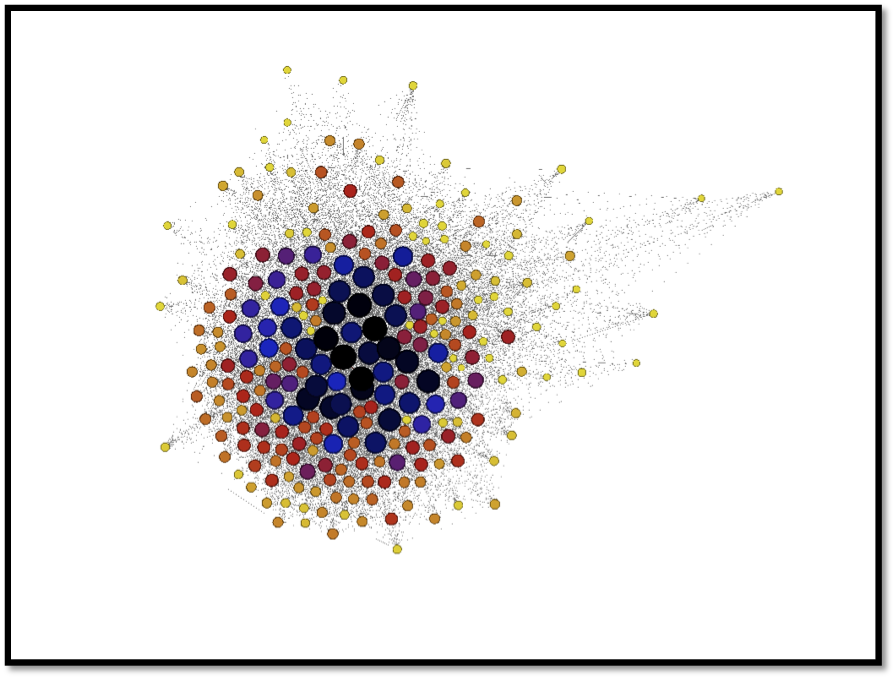
\includegraphics[scale=0.7]{img/7/grafo12}
\caption{Relaciones entre etiquetas.
\label{fig:grafo12}}
\end{figure}

Otro grafo más simplificado se muestra en la figura~\ref{fig:grafo14}, con las siguientes características:
\begin{itemize}
\item    El grafo tiene 21 nodos y 86 aristas.
\item    Los nodos están escalados según su grado nodal (número de relaciones con otras etiquetas).
\item    Las aristas están escaladas según su peso (número de ocurrencias de esa relación).
\item    Aparecen 2 comunidades en el grafo: color del nodo (turquesa y rojo).
\item    El grado nodal medio del grafo es 8,19.
\item    Sólo hay 1 componente conexa.
\end{itemize}

\begin{figure}
\centering
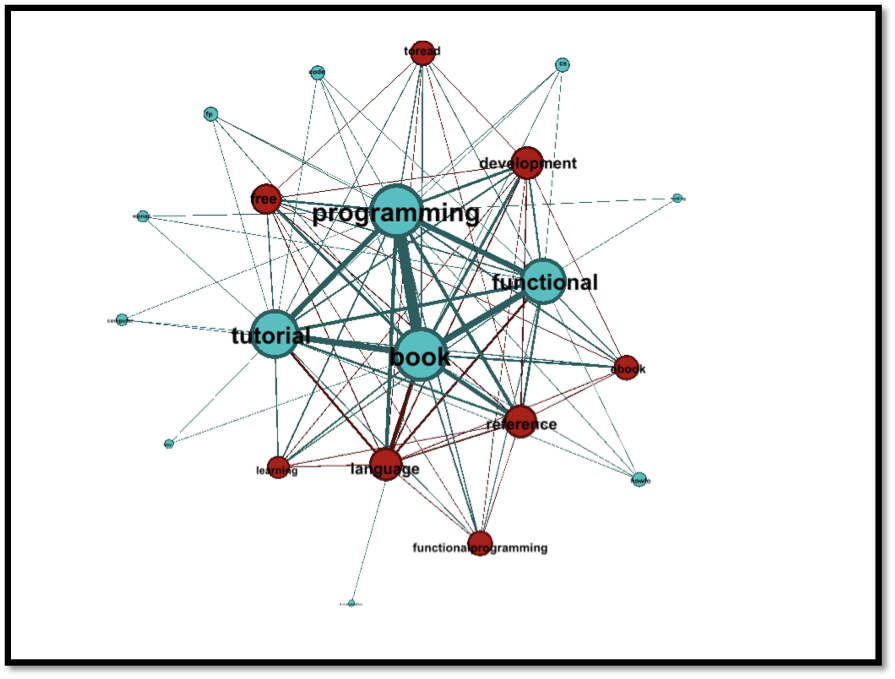
\includegraphics[scale=0.7]{img/7/grafo14}
\caption{Relaciones entre etiquetas (simplificado).
\label{fig:grafo14}}
\end{figure}

La generación de este nodo simplemente es un proceso de simplificación en el que se eliminan los nodos con menor grado nodal con respecto al grafo anterior.





\subsection{Relaciones entre usuarios (por lenguaje común).}

Este grafo presenta las relaciones entre los {\bf usuarios} del sistema, en función de su {\bf lenguaje común}; es decir, el número de etiquetas comunes con otros usuarios.

\subsubsection{Representación.}

Este grafo tiene como puntos de partida:

\begin{itemize}
\item    Los nodos corresponden a los usuarios del sistema.
\item    El peso de los nodos es el tamaño del lenguaje de dicho nodo (usuario); es decir, el número de etiquetas que usa dicho usuario.
\item    Las aristas representan relaciones entre dos usuarios (dos nodos). Esta relación existirá cuando posean algún lenguaje común; es decir, que compartan alguna etiqueta (aunque dicha etiqueta no esté en los mismos enlaces para ambos). Otra forma de verlo sería decir que existe una arista entre dos usuarios cuando la interesección de sus conjuntos de etiquetas es no vacía.
\item    El peso de las aristas es el número de etiquetas que forman parte de dicha intersección.
\end{itemize}

\subsubsection{Resultado.}

El grafo obtenido tiene las siguientes características:

\begin{itemize}
\item    El número de nodos es 4259.
\item    El número de aristas es 6844837.
\item    El grado nodal máximo del grafo es 4178; es decir, existe un usuario cuyo lenguaje (conjunto de etiquetas) contiene alguna etiqueta en común con el lenguaje de otros 4178 usuarios.
\item    El grado nodal medio del grafo es 1607.1465
\item    El peso nodal máximo es 238; es decir, un usuario que ha etiquetado con 238 etiquetas diferentes, y ese es el número máximo de nuestro sistema.
\item    El peso nodal medio es $7.3575954$.
\item    El peso de arista máximo es 64; es decir, existe un par de usuarios cuya intersección de lenguajes (conjunto de etiquetas comunes) está formada por 64 etiquetas, y este par de usuarios es el que tiene una intersección más grande.
\item    El peso medio de las aristas es de $2.0418215$
\item Los nodos más destacables son \emph{{\bf 75: airlab.am}} ($peso=238$), \emph{{\bf 47: MC Andre}} ($peso=192$), \emph{{\bf 11: Tang Tong}} ($peso=167$), \emph{{\bf 104: Matthew}} ($peso=141$) y \emph{{\bf 3002: timcowlishaw}} ($peso=134$).
\item Las aristas más destacables son \emph{{\bf 75-104}} ($peso=64$), \emph{{\bf 11-75}} ($peso=56$), \emph{{\bf 11-104}} ($peso=53$), \emph{{\bf 75-1659}} ($peso=46$) y \emph{{\bf 75-115}} ($peso=43$). Estas aristas expresan los IDs de los usuarios en el sistema.
\end{itemize}

\subsubsection{Simplificación del grafo.}

Se llevan a cabo las siguientes tareas para simplificar el grafo:

\begin{itemize}
\item    Un primer proceso de filtrado consistirá en eliminar todos aquellos nodos cuyo peso nodal sea menor que el peso nodal medio del grafo (que es $7.3575954$). Esta operación, además de eliminar estos nodos, elimina también todas las aristas cuyo origen o destino tiene a este nodo. Recuérdese que el peso nodal se corresponde con el tamaño del lenguaje del usuario representado por dicho nodo; es decir, el número de etiquetas diferentes que ha usado en el etiquetado. Por tanto, con este filtrado se eliminarán a todos aquellos usuarios cuyo lenguaje tenga menos de 8 etiquetas diferentes.
\item    Un segundo proceso de filtrado consistirá en eliminar todas aquellas aristas cuyo peso sea menor que el peso medio de arista del grafo (que es $2.0418215$). Recuérdese que el peso de arista se corresponde con el tamaño del lenguaje común de un par de usuario (usuario del nodo origen y usuario del nodo destino); es decir, el número de etiquetas distintas que son usadas por ambos usuarios. Por tanto, con este filtrado se eliminarán a todos aquellos pares de usuarios cuyo lenguaje común tenga menos de 3 etiquetas comunes.
\item A continuación, se repetirá el proceso de filtrado de aristas que no superen el nuevo peso medio de arista obtenido tras el proceso anterior. Este nuevo valor es $4.144222$.
\item Finalmente, se eliminan las aristas menos significativas (aquellas con menor peso), y todos los nodos que pasen a tener grado nodal 0.
\end{itemize}


\subsubsection{Grafo resultante.}

El grafo resultante se muestra en la figura~\ref{fig:grafo33}. Algunas características de este grafo son:

\begin{itemize}
\item    Los nodos son usuarios, se incluye el nombre de cada usuario.
\item    El tamaño del nodo está escalado según su grado nodal; es decir, según el número de otros usuarios con los que tiene relación. Su nombre está igualmente escalada.
\item    Las aristas son relaciones entre dos usuarios.
\item    La anchura de las aristas está escalada según su peso; es decir, según el tamaño del lenguaje común que representa dicha aristas.
\item    Los nodos y las aristas están coloreados según las comunidades a las que pertenecen, existiendo 4 comunidades diferentes.
\end{itemize}

\begin{figure}
\centering
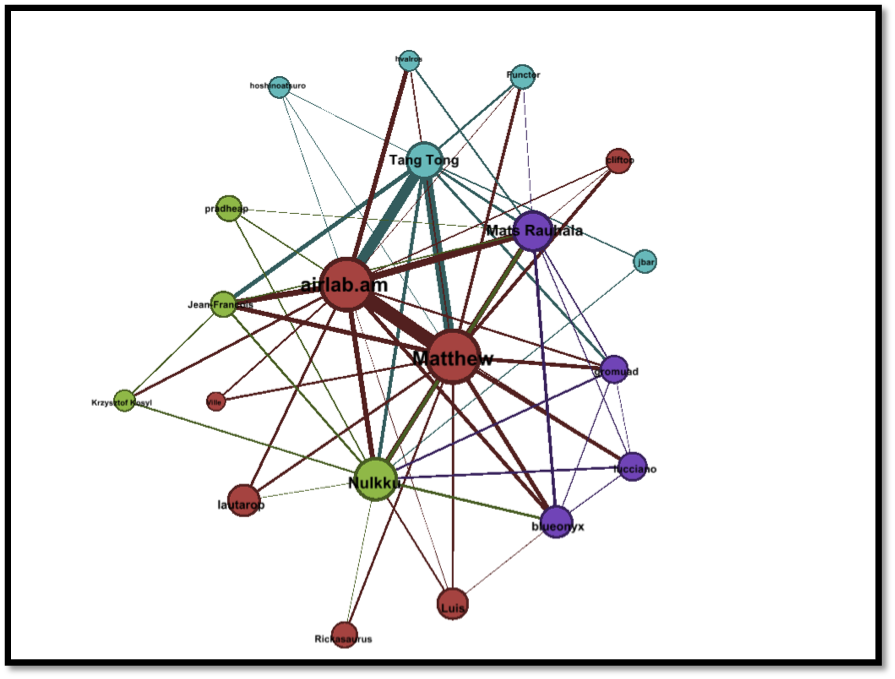
\includegraphics[scale=0.7]{img/7/grafo33}
\caption{Relaciones entre usuarios (por lenguaje común).
\label{fig:grafo33}}
\end{figure}








\subsection{Relación entre usuarios (por contextos comunes).}

Este grafo, muy similar al anterior, presenta las relaciones entre los {\bf usuarios} del sistema, en función de los {\bf contextos comunes} que tienen entre ellos; es decir, el número de enlaces comunes con otros usuarios.

\subsubsection{Representación.}

Este grafo tiene como punto de partida:

\begin{itemize}
\item    Los nodos corresponden, igual que en el grafo anterior, a los usuarios del sistema.
\item    El peso de los nodos es el tamaño del contexto de dicho nodo (usuario); es decir, el número de enlaces que tiene etiquetado dicho usuario.
\item    Las aristas representan relaciones entre dos usuarios (dos nodos). Esta relación existirá cuando posean algún contexto común; es decir, que compartan algún enlace (aunque dicho enlace no tenga la misma etiquetación para ambos). Otra forma de verlo sería decir que existe una arista entre dos usuarios cuando la interesección de sus conjuntos de enlaces es no vacía.
\item    El peso de las aristas es el número de enlaces que forman parte de dicha intersección.
\end{itemize}

\subsubsection{Resultado.}

El grafo obtenido tiene las siguientes características:
\begin{itemize}
\item    El número de nodos es 4259. Igual que para el grafo anterior.
\item    El número de aristas es 616708. Se observa que este número es mucho menor que en el grafo anterior, ya que es más difícil que dos usuarios compartan enlaces a que compartan etiquetas.
\item    El grado nodal máximo del grafo es 1877; es decir, existe un usuario cuyo contexto (conjunto de enlaces) contiene algún enlace en común con el lenguaje de otros 1877 usuarios.
\item    El grado nodal medio del grafo es $144.80113$.
\item    El peso nodal máximo es 111.
\item    El peso nodal medio es $2.3944588$
\item    El peso de arista máximo es 11; es decir, existe un par de usuarios cuya intersección de contexto (conjunto de enlaces comunes) está formada por 11 enlaces, y este par de usuarios es el que tiene una intersección más grande.
\item    El peso medio de las aristas es de $1.0205121$.
\item Los nodos más destacables que en el caso anterior: \emph{{\bf 75: airlab.am}} ($peso=238$), \emph{{\bf 47: MC Andre}} ($peso=192$), \emph{{\bf 11: Tang Tong}} ($peso=167$), \emph{{\bf 104: Matthew}} ($peso=141$) y \emph{{\bf 3002: timcowlishaw}} ($peso=134$).
\item Las aristas más destacables son: \emph{{\bf 104-105}} ($peso=11$), \emph{{\bf 104-331}} ($peso=9$), \emph{{\bf 11-104}} ($peso=8$), \emph{{\bf 104-215}} ($peso=7$) y \emph{{\bf 104-796}} ($peso=7$).
\end{itemize}

\subsubsection{Simplificación y grafo resultante.}

Al igual que en el proceso anterior, se han eliminado las aristas menos significativas (según su peso), para que la representación sea amigable, dejando únicamente visibles en el siguiente grafo las aristas más significativas del sistema. En este proceso de filtrado se han eliminado todas aquellas aristas con peso menor que 5; es decir, se han eliminado todos los pares de usuarios que comparten menos de 5 enlaces en su contexto común. Obviamente, se han eliminado también los nodos que, tras la eliminación de estas aristas, han quedado con grado nodal igual a 0; es decir, sin relaciones con ningún otro usuario.

También se han escalado los nodos según su grado nodal (y también los nombres de éstos), las aristas según su peso, y se han coloreado tanto nodos como aristas en función de las comunidades obtenidas.

El grafo resultante se puede ver en la figura~\ref{fig:grafo42}.

\begin{figure}
\centering
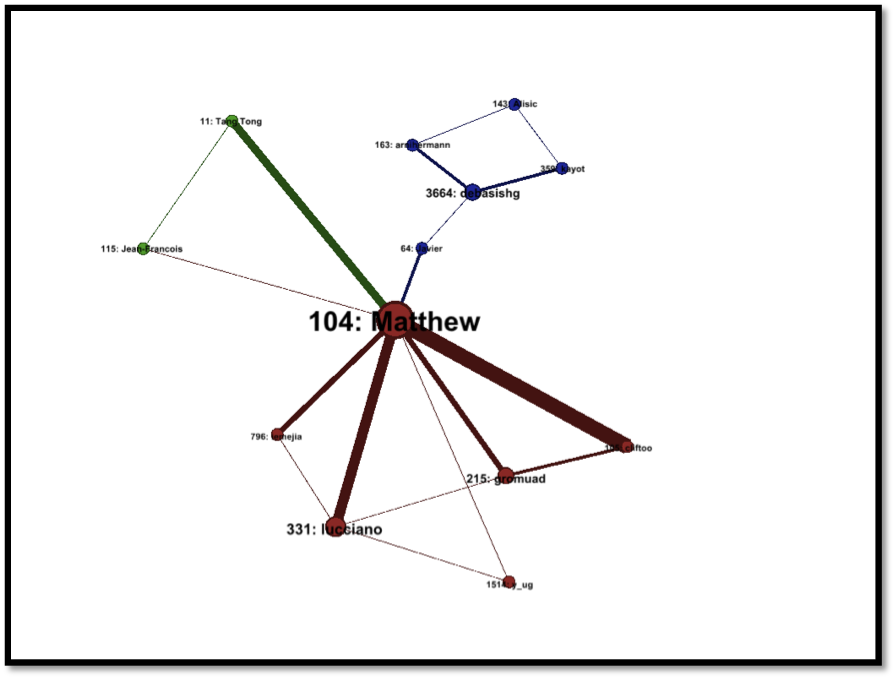
\includegraphics[scale=0.7]{img/7/grafo42}
\caption{Relaciones entre usuarios (por contexto común).
\label{fig:grafo42}}
\end{figure}


\section{Ejecución del SMA.}

Como se comentó en el capítulo~\ref{cap:capitulo6}, se ha realizado una ejecución del sistema con umbrales iguales o superiores a 3. Para optimizar las ejecuciones, cada ejecución se ha ceñido a calcular aquellas conciliaciónes de un valor concreto; es decir, que sólo se realizarán conciliación de conceptos entre aquellos usuarios que compartan exactamente el número de objetos marcados por el valor de \emph{umbral}. Sin embargo, todos los resultados se almacenan en una base de datos de forma conjunta, de forma que se puedan sacar conclusiones a posteriori.

De esta forma, se ha realizado un pequeño script, en el que se obtienen los siguientes resultados (ver tabla~\ref{fig:resultados}), tanto totales, como separados por los diferentes posibles valores de \emph{umbral}. Hay que indicar que este proceso realiza un cálculo del número de conceptos y el número de implicaciones de cada contexto encontrado. Estos contextos son, precisamente, los contextos comunes resultados de alguna conciliación tras la ejecución del SMA. Los datos que se adjuntan se refieren a estos valores por cada contexto conciliado.

Finalmente, hay que indicar que no se ha realizado con umbrales inferiores a 3 por cuestiones de implementación, tal como se comentaba en el capítulo anterior.

\begin{figure}
\centering
{ \scriptsize
\begin{tabular}{|l|c|c|c|c|c|c|c|c|c|c|}
\hline
& Total 
&\begin{sideways} Umbral=3 \end{sideways} 
&\begin{sideways} Umbral=4 \end{sideways} 
&\begin{sideways} Umbral=5 \end{sideways} 
&\begin{sideways} Umbral=6 \end{sideways} 
&\begin{sideways} Umbral=7 \end{sideways} 
&\begin{sideways} Umbral=8 \end{sideways} 
&\begin{sideways} Umbral=9 \end{sideways} 
&\begin{sideways} Umbral=10 \end{sideways} 
&\begin{sideways} Umbral=11 \end{sideways} 
 \\ \hline

Nº Conciliaciones & 663 		& 561 	& 75 		& 15 		& 7 		& 2 		& 1 		& 1 & 0 &  1   \\ \hline
Media Objetos 	& $33.546$ 	& $28.742$ & $52.76$ & $76.667$ & $71.714$ & 87 	& 144 	& 92 & - &  98   \\ \hline
Total Objetos & 22241 		& 16124 	& 3957 	& 1150 	& 502 	& 174 	& 144 	& 92 &-  &  98 \\ \hline
Máx Objetos & 144 			& 130 	& 117 	& 138 	& 86 		& 97 		& 144 	& 92 & - &  98   \\ \hline
Media Lenguaje & $9,413$ 		& $8.234$ 	& $13.2$ 	& $24$ 	& 12 		& 30 		& 53 		& 38 & - &  37   \\ \hline
Total Lenguaje & 6241 		& 4619	& 990	& 360	& 84 		& 60 		& 53 		& 38 & - &  37   \\ \hline
Máx Lenguaje & 64 			& 43 		& 42 		& 64 		& 26 		& 38 		& 53 		& 38 & - &  37   \\ \hline
Media Conceptos & $6.092$ & $5.365$ 	& $7.867$ 	& $15.333$ & 10 	& $26.5$ 	& 32 		& 25 & - &  29   \\ \hline
Total Conceptos & 4039 	& 3010 	& 590 	& 230 	& 70 		& 53 		& 32 		& 25 & - &  29   \\ \hline
Máx Conceptos & 40 		& 40 		& 26 		& 38 		& 23 		& 32 		& 32 		& 25 & - &  29   \\ \hline
Media Implicaciones & $9.75$ & $7,957$ & $14.653$ & $34,467$ & $15.143$ & $45.5$ & 80 	& 51 & - &  56   \\ \hline
Total Implicaciones & 6464 	& 4464 	& 1099 	& 517 	& 106 	& 91 		& 80 		& 51 & - &  56   \\ \hline
Máx Implicacioens & 114 	& 71 		& 58 		& 114 	& 38 		& 50 		& 80 		& 51 & - &  56   \\ \hline
\end{tabular}
}
\caption{Resultados de la Ejecución del SMA
\label{fig:resultados}
}

\end{figure} 






\section{Resultados estadísticos y Conclusiones.}

En la figura~\ref{fig:estNConc} se puede observar una gráfica del número de conciliaciones en función del umbral. En esta gráfica se observa un decrecimiento exponencial del número de conciliaciones a medida que aumenta el umbral. Esto tiene sentido ya que el número de usuarios que quieren conciliar su conocimiento con otros usuarios aumentará a medida que se reduce este umbral de objetos comunes. En los umbrales más altos, se ve como el número de conciliaciones tiende a cero. Añadir, además, que no se adjuntan datos para las conciliaciónes con umbral igual a 0, 1 y 2; porque no se ha implementado en el sistema.

%\begin{figure}
%%\centering
%
%\begin{minipage}[b]{0.42\linewidth}
%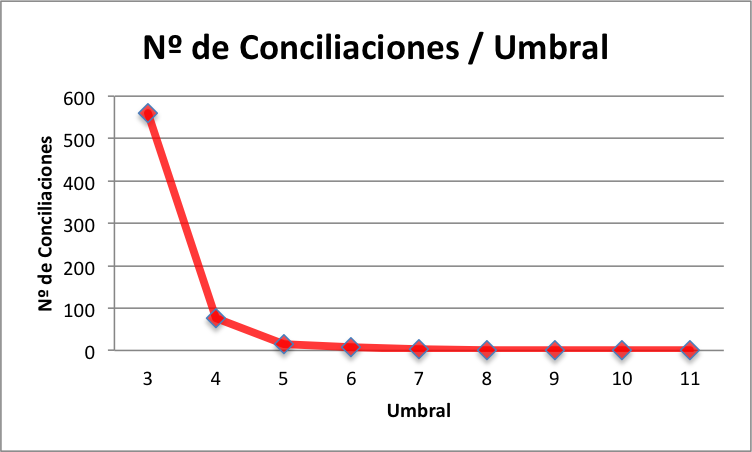
\includegraphics[scale=0.47]{img/7/est_nconciliaciones}
%\end{minipage}
%\hspace{0.1cm}
%\begin{minipage}[b]{0.42\linewidth}
%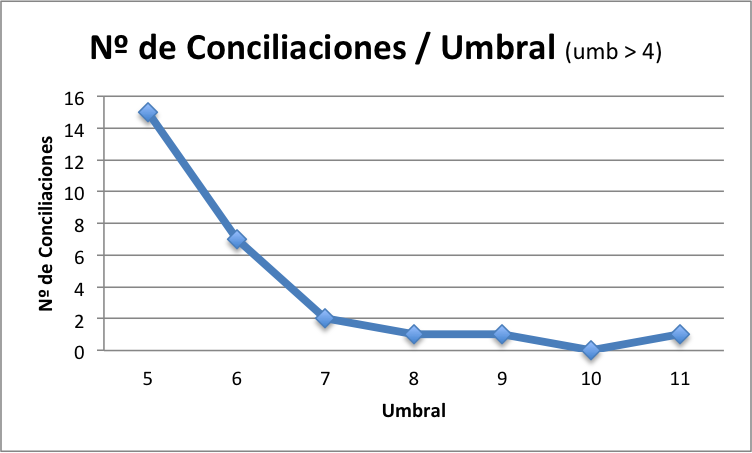
\includegraphics[scale=0.56]{img/7/est_nconciliaciones2}
%\end{minipage}
%
%\caption{Número de conciliaciones por umbral.
%\label{fig:estNConc}}
%\end{figure}

\begin{figure}
\centering

\begin{minipage}[b]{0.45\linewidth}
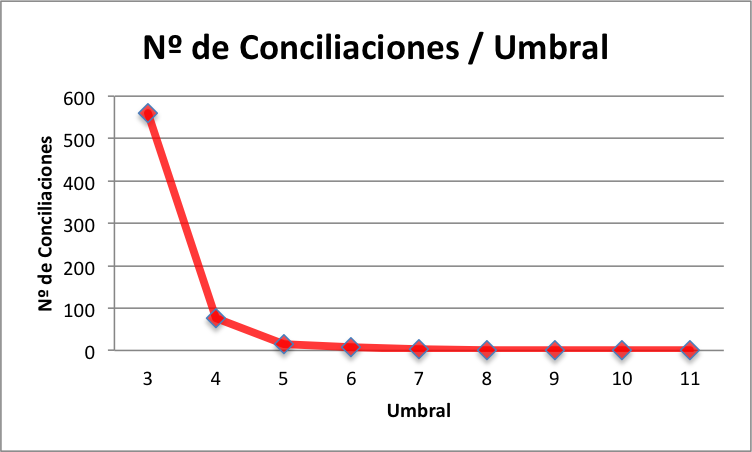
\includegraphics[scale=0.5]{img/7/est_nconciliaciones}
\end{minipage}
\hspace{0.3cm}
\begin{minipage}[b]{0.45\linewidth}
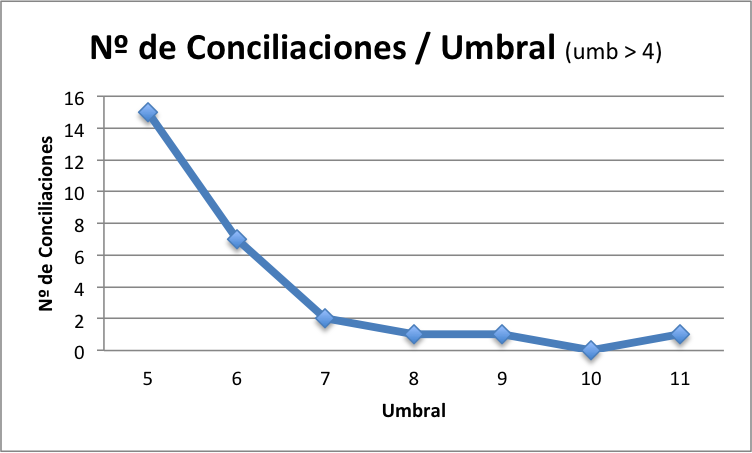
\includegraphics[scale=0.5]{img/7/est_nconciliaciones2}
\end{minipage}

\caption{Número de conciliaciones por umbral.
\label{fig:estNConc}}
\end{figure}

En la figura~\ref{fig:estObj} se puede observar una doble gráfica sobre el número de objetos comunes y el número de atributos comunes por contexto conciliado en función del umbral. Estos valores son la media de todos los contextos conciliados para dicho umbral. Se ve como inicialmente, los contextos generados poseen muy pocos objetos y atributos, por lo que son contextos muy pobres. Esto se explica ya que cuando dos usuarios tienen pocos objetos en común, es también probable que su lenguaje común sea reducido; y por tanto, la conciliación apenas genere nuevas sugerencias. En cambio, a medida que los umbrales aumentan; es decir, a medida que los usuarios comparten más objetos, se observa una tendencia de contextos más ricos en cuanto a número de objetos y número de atributos. Sin embargo, lo más importante es notar esta tendencia, ya que los valores numéricos no son significativos puesto que el número de contextos conciliados no es muy elevado.

\begin{figure}
\centering
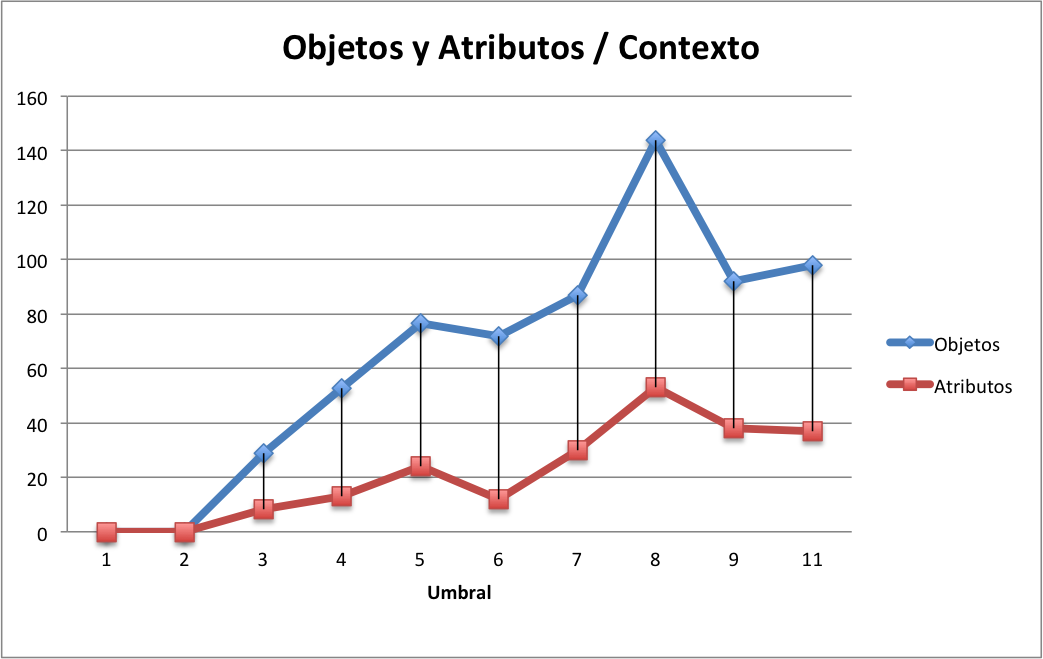
\includegraphics[scale=0.75]{img/7/est_nobj}
\caption{Número medio de Objetos y Atributos por Contexto conciliado según Umbral.
\label{fig:estObj}}
\end{figure}

Finalmente, en la figura~\ref{fig:estconceptos} se puede observa una doble gráfica sobre el número de conceptos y el número de implicaciones por contexto conciliado en función del umbral. Estos valores son la media de todos los contextos conciliados para cada uno de estos umbrales. Igual que en el caso anterior, se obseva una tendencia positiva en cuanto al crecimiento de número de conceptos y número de implicaciones generados por contexto conciliado a medida que aumenta el umbral; es decir, a medida que los pares de usuarios que concilian su conocimiento comparte un mayor número de enlaces. Es interesante destacar que en los últimos umbrales se producen algunas desviaciones en esta tendencia. Esto es debido a que el número de conciliaciones es muy reducido (1 o 2 según el caso), por lo que no representan una muestra representativa para tomar valores exactos. Sin embargo, muestran perfectamente esta tendencia creciente.

\begin{figure}
\centering
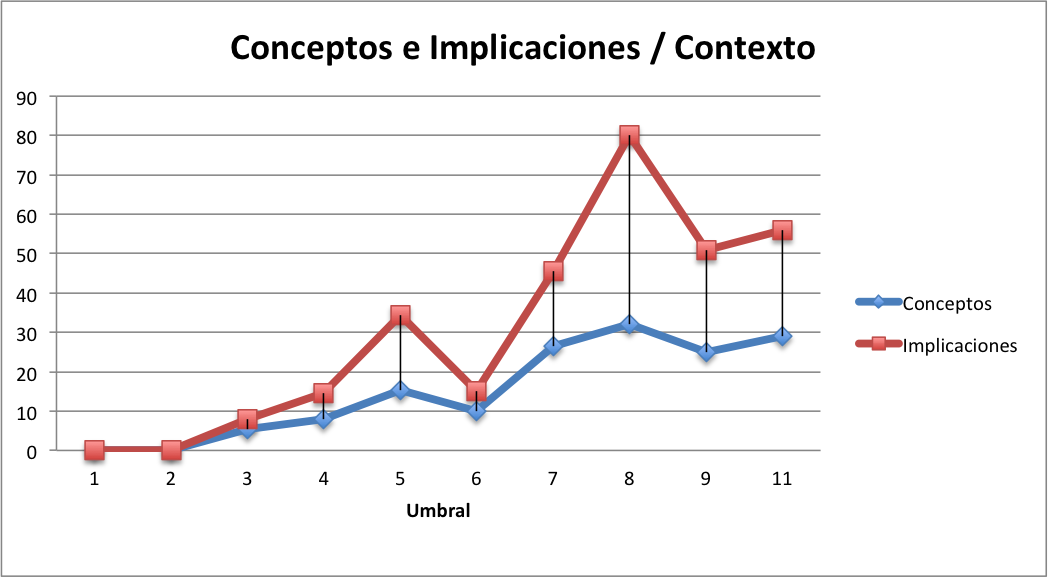
\includegraphics[scale=0.75]{img/7/estconceptos}
\caption{Número medio de Conceptos e Implicaciones por Contexto conciliado según Umbral.
\label{fig:estconceptos}}
\end{figure}